\newcommand{\TODO}[1]{\textbf{TODO: #1}} \newcommand{\eg}{\emph{e.g.}}
\newcommand{\ie}{\emph{i.e.}}
\newcommand{\mypara}[1]{\textbf{#1}}

\section{Introduction} \label{sec:introduction}

This paper presents a \emph{safe} and \emph{efficient} region-based approach
to \emph{data transferable} between a set of concurrent actors, motivated by the following concerns.

Consider the example (of  a producer creating a data structure and transferring it to a consumer)
in Fig.~\ref{fig:motivating-eg}.
This represents a \C{SELECT} query operator that receives a stream of input messages,
each associated with a time window $t$, processed by method \texttt{onReceive}.
Each input message contains a list of inputs, each processed by applying a user-defined function to
create a corresponding output.  Multiple messages with the same timestamp
are permitted and messages with different timestamps may arrive out of order.
An invocation of method
\texttt{OnNotify} indicates that no more input messages with a timestamp
$t$ will be subsequently delivered.  At this point, the operator completes
the processing for time window $t$ and sends a corresponding output message
to its successor.

\begin{figure}[t!]
\begin{numcodejava}
class MapVertex<TIn, TOut> {
  Func<TIn, TOut> selector;
  Dictionary<Time, List<TOut>> map;
  ...
  void onReceive(Time t, List<TIn> inputs) {
    if (!map.ContainsKey(t))
       map[t] = new List<TOut>();
    foreach (TIn input in inputs) {
      TOut output = selector(input);
      map[t].add(output);
    }
  }
  void onNotify(Time t) {
     List<TOut> outputList = map[t];
     map.Remove(t);
     transfer(successorId, t, outputList); 
  }
}
\end{numcodejava}
\caption{\C{SELECT} dataflow operator}
\label{fig:motivating-eg}
\end{figure}


\mypara{Performance.}
When the transferred data structures are large, as is the case with many
streaming big-data analysis systems, garbage collection overhead becomes
significant~\cite{Broom:HotOS}.  Further, in a distributed
dataflow system, the GC pause at one node can have a cascading adverse
effect on the performance of other nodes~\cite{Broom:HotOS,harris15}:
a GC pause at an upstream actor can block downstream actors that are waiting for
messages.  However, much of the GC overhead results from the
collector performing avoidable or unproductive work.  For the example
in Fig.~\ref{fig:motivating-eg}, GC might repeatedly traverse the
\C{map}, although its objects cannot be collected until a
suitable timing message arrives.
There has been increasing interest in off-heap memory management for better performance
in the context of several  systems and languages (e.g.,
Spark~\cite{SPARK:2015}, Scala~\cite{ScalaOffHeap}, Rust).
Several systems (e.g.,~\cite{TRILL:2014}) resort to using ``free object pools'' to partially alleviate this problem, in
the absence of language support.

\begin{figure}
\centering
\subcaptionbox {
  Before transfer.
  \label{fig:after-transfer}
} [
  0.35\columnwidth
] {
  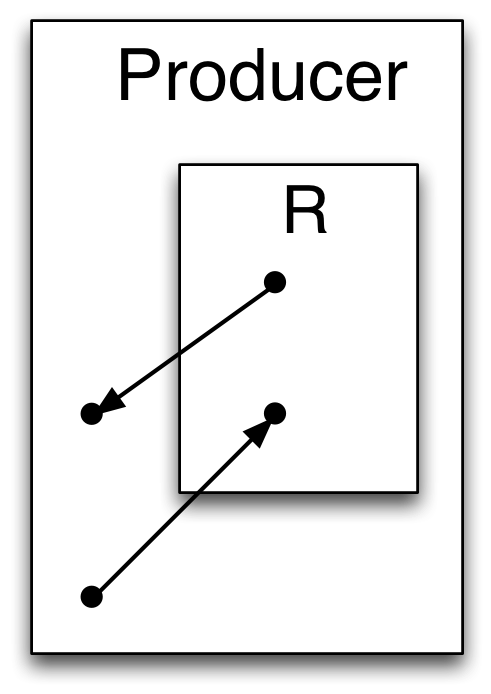
\includegraphics[scale=0.36]{producer-heap}
}
\subcaptionbox {
  After transfer.
  \label{fig:before-transfer}
} {
  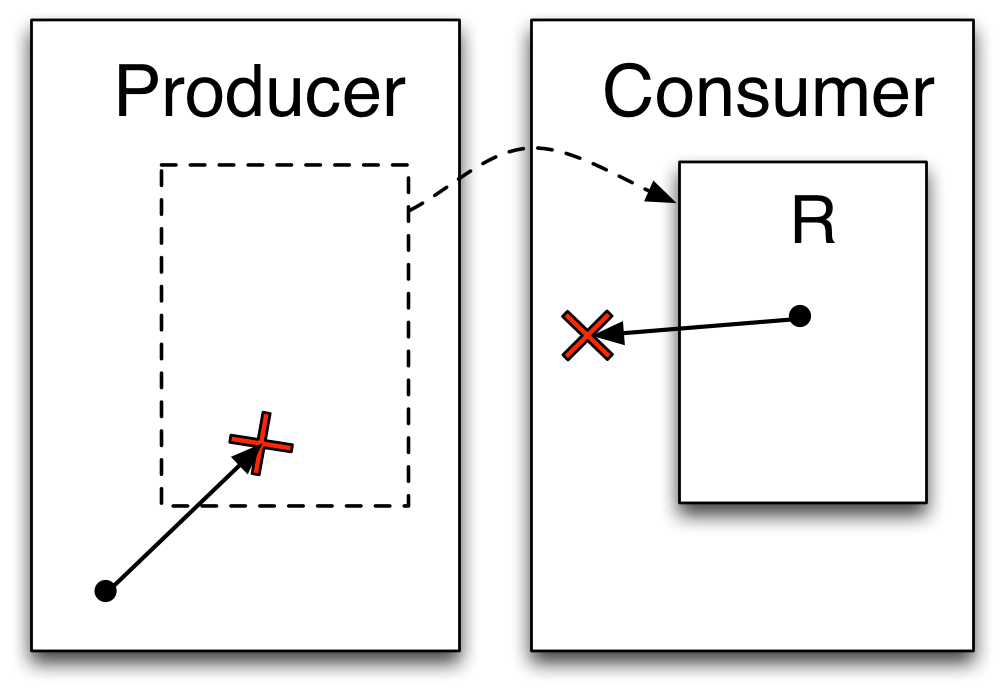
\includegraphics[scale=0.36]{producer-consumer-heap}
}

\caption{References in and out of a transferable region ($R$) become
invalid after transfer.}
\label{fig:transfer-violations}
\end{figure}

\mypara{Safety.}
Several of these systems are designed to allow the producer and consumer to
execute in the same address space or in different address spaces
(as determined by the compiler and runtime).
We wish to ensure memory safety in the presence of such transferred data.
% by ensuring that there are no invalid references.
A transfer operation, with no
additional checks, may cause memory safety violations, both at the
producer of the data structure, and its (possibly remote) consumer. At
the producer, any existing references into the transferred data structure become
invalid post transfer. If the data structure contains references to
objects outside (the transferred data), then such references become
invalid in the context of the consumer. Both scenarios are depicted in
Fig.~\ref{fig:transfer-violations}.
% Safety violations of this kind are
% particularly unwelcome in the context of languages like C\# and Java
% that are otherwise memory-safe.
While references from within the transferable data to outside can be disallowed
in the interest of safety,
references into transferable data needs to be allowed before the data
is transferred. Allowing such references is crucial, % to performance,
as any non-trivial program creates temporary references to the internal
objects of a data-structure.

\mypara{Safe Transferable Regions.}
In this paper, we present a language-based approach to cleanly encapsulated
transferable data and a safe and efficient implementation of such data based
on regions. 
%
A region is a block of memory that is allocated
and freed in one shot, often in constant time. A region may contain
one or more contiguous range of memory locations, and individual
objects may be dynamically allocated within the region over time,
while they are deallocated en masse when the region is freed.  Thus, a
region is a good fit for a transferable data-structure.  In
Fig.~\ref{fig:motivating-eg}, the output to be constructed for each
time window $t$ (i.e., \C{map[t]}) can be a separate region that is
allocated when the first message with timestamp $t$ arrives, and
deallocated after \C{map[t]} is transferred in \C{onNotify}.

The use of regions alleviates the performance concern related to
garbage collection described earlier. (It also enables more efficient
serialization/deserialization of data-structures across address spaces,
which is also a significant performance bottleneck in such systems.)
However, manual region memory management introduces memory safety
issues such as dangling pointers.
We present a single type system that simultaneously addresses
this safety concern, as well as those described above related to
the use of \emph{transferable data}.

% Region-based memory management, both manual as well as automatic, has
% been known for a long time. Manual region-based memory management
% suffers from the usual drawbacks, namely the potential for invalid
% references and the consequent lack of memory safety. Automatic
% region-based memory management systems guarantee memory safety, but
% impose various restrictions.  MLKit, which implements the approach
Safe region-based memory management using types was
pioneered by Tofte and Talpin~\cite{tofte94,tofte97}, who 
use only lexically scoped regions.  At runtime, the set of all regions
(existing at a point in time) forms a stack. Thus, the lifetimes of
all regions must be well-nested: it is not possible to have two
regions whose lifetimes overlap, with neither one's lifetime contained
within the other.  Unfortunately, the data structures in the above
example do not satisfy this restriction (as the output messages for
multiple time windows may be simultaneously live, without any
containment relation between their lifetimes).  We refer to regions
with lexically scoped lifetimes as \emph{stack regions} and to regions
that do not have such a lexically scoped region as \emph{dynamic}
regions.

Our focus, in this paper, is on first-class \emph{memory-safe} dynamic regions
that can be safely transferred across address spaces. We refer to such dynamic
regions as \emph{transferable} regions.
%
Our approach is based on a variation of ideas introduced by~\cite{WW01,cyclone04}
that combine linear types and regions to support dynamic regions.
Unlike the prior work, we ensure memory safety in the presence of
transferable regions through a \emph{combination of a static
typing discipline and lightweight runtime checks in place of linear types}.

\mypara{Language.}
The cornerstone of this approach is an \C{open} lexical block for transferable regions,
that ``opens'' a transferable region and guarantees that the region
won't be transferred/freed while it is open. By nesting a
Tofte-Talpin style \C{letregion} lexical block, that delimits
the lifetime of a stack region, inside an \C{open} lexical block for a
transferable region, we can guarantee that the transferable region
will remain live as long as the stack region is live. We say that the
former \emph{outlives} the later., and any references from the stack
region to the transferable region are therefore safe.
This is particular useful, since such stack regions serve as temporary
working storage while working with the (opened) transferable regions.

By controlling the outlives relationships between various
regions, we only allow safe cross-region references, while prohibiting
unsafe ones. In the above example, an outlives relationship
\emph{from} the stack region \emph{to} the transferable region means
that the references in that direction are allowed, but not the
references in the opposite direction. In contrast, if an \C{open}
block of a transferable region $R_0$ is nested inside an \C{open}
block of another transferable region $R_1$, we do not establish any
outlives relationships, thus declaring our intention to not allow any
cross-region references between $R_0$ and $R_1$.  Finally, we observe
that outlives relationships are established based on the lexical
structure of the program, hence a static type system can enforce them
effectively. By assigning region types to objects, which capture the
regions such objects are allocated in, and by maintaining outlives
relationships between various regions, we can statically decide the
safety of all references in the program.

\mypara{Type System.}
Formally, our type system introduces \emph{region parameters} (for both
classes and methods) and uses constrained parametric polymorphism
over these parameters, where the constraints capture outlives constraints
between the region parameters.
The type system may be seen as a form of ownership type system~\cite{OwnershipSurvey},
with a region being the owner of all objects allocated in that region.

\mypara{Lightweight Runtime Checks.}
Ensuring memory safety using this approach requires ensuring
that the use of transferable regions satisfies certain temporal properties.
Firstly, a transferable region should not be transferred/freed
inside an open block of that region (i.e, while it is still open).
Secondly, a transferred/freed region should not be opened. These are
typestate invariants on the transferable region objects, which are
hard to enforce statically in the presence of unrestricted
aliasing. Techniques like linear types and unique pointers can be used
to restrict aliasing, but the constraints they impose are often hard
to program around. We therefore enforce typestate invariants at
runtime via lightweight checks. In particular, we define an acceptable
state transition discipline for transferable regions
(Fig.~\ref{fig:region-fsm}), and check, at runtime, whether a given
transition of a transferable region (\eg, from \emph{open} state to
\emph{freed} state) is valid or not. The check is lightweight since it
only involves checking a single tag that captures the current state.
We believe that this is a reasonable choice since regions are
coarse-grained objects manipulated infrequently, when compared to the
fine-grained objects that are present inside these regions, for which
safety is enforced statically. 

\mypara{Type Inference.}
One of the key contributions of this paper is a sound type inference algorithm
that eliminates the need for users to write region type annotations.
The users write programs in the underlying language that provides
primitives for the users to manipulate regions (create, open, free,
transfer) and to allocate objects in regions, but has no region type
annotations.
% This, we believe, significantly reduces the impediment to adopt our
% approach in practical setting.

Our inference algorithm proceeds in three stages: in the first stage,
we elaborate the program by introducing region parameters (for classes
and methods); in the second stage we generate a set of constraints
that must be satisfied for the program to type check; in the third
stage, we solve the set of constraints, inferring the preconditions of
all classes and methods (in terms of the expected outlives-constraints
between the region parameters).  We show that the algorithm is sound,
and the last stage of constraint solving is complete.
% (using an interprocedural fixed point computation).

\mypara{Evaluation.}
Our work was inspired by~\cite{Broom:HotOS}, which presents evidence that
realistic programs can be written using transferable regions
and that this can yield significant performance improvements.
The system described in~\cite{Broom:HotOS}, however, provides no memory
safety guarantees, which is the subject of our contribution.
We report on an implementation of our type inference algorithm that
was able to identify some unsafe memory accesses and was able to successfully
verify programs correct (once the errors were fixed).

% transferableally checking for the second category of
% invariants is easy and does not pose a performance concern (unlike,
% \eg, the first category of constraints); a static typechecker that
% rules out the second category of violations would be very restrictive
% from an expressiveness perspective; finally, the human effort required
% to ensure the second set of invariants is not as burdensome (as
% regions are coarse-grained objects manipulated infrequently), \eg, as
% it would be for the first set of invariants.

% when a producer transfers a
% region containing a data structure to a consumer, in a shared-memory
% context, we enforce an ownership discipline that ensures that the
% producer cannot subsequently modify the data structure. When the same
% transfer happens in a distributed setting, we guarantee that (a). the
% data structure is contained in the region, and can be safely
% transmitted across address spaces, and (b). once the transfer
% concludes, the producer can safely deallocate the memory for the
% data structure without the fear of violating memory safety.

%  Transfer operation,
% with no additional checks and balances, may cause memory safety
% violations, both at the producer of the data structure, and the
% (possibly remote) consumer of the data structure. A key invariant and restriction
% that we utilize
% to achieve this is that no object $o_1$ in one transferable region $D_1$
% can contain a pointer to an object $o_2$ in another transferable region
% $D_2$.  In cases where this is too restrictive, the user has to resort
% to (deep) copying $o_2$ to $D_1$.  This is conceptually quite
% reasonable given the perspective that $D_1$ is a self-contained
% data structure.  Furthermore, this is quite analogous, from a
% performance perspective, to the copying that happens when a garbage
% collector promotes an object from a lower generation to a higher
% generation.  From this perspective, a region may be seen as a
% user-controlled generation.

% This ensures that we can safely free one transferable region (\eg, the
% input-message in our example) without affecting the validity of
% pointers in another transferable region (\eg, the output-message).
% However, this is not sufficient! When processing the input-message
% $D$, we necessarily will have to create pointers that point to objects
% that are internal to $D$. Such pointers may be stack-allocated or even
% reside in the heap (\eg, consider the iterator object used to iterate
% over the list in the input-message).  How do we ensure the safety of
% these pointers?

% We use \emph{stack regions} (regions with lexically-scoped lifetimes),
% as well as the stack, for such temporary pointers (to objects inside a
% transferable region) and use the following protocol to ensure safety
% of such pointers.  To work with a transferable region $D$, we must
% first \emph{open} the region $D$, to indicate that $D$ should not be
% freed during this period. When the processing of the region is
% complete, we \emph{close} the region $D$, to indicate that it is safe
% to free $D$.  In general, a transferable region may be opened and
% closed multiple times before it is eventually transferred or freed.

% Our type-system permits the creation of pointers to internal objects
% of \emph{open transferable} regions, but uses lexical scoping to ensure
% that such pointers are no longer live when the region is closed.
% Thus, such pointers may be either stack-allocated or reside in a
% region whose lifetime is statically guaranteed to be contained within
% the interval when $D$ is open.  As a consequence, the system ensures
% the strong invariant that for a \emph{closed transferable} region $D$ no
% pointer from outside $D$ points to an internal object of $D$.

% The final piece required to ensure memory-safety is ensuring that the
% program correctly follows the above-mentioned protocol for transferable
% regions: \eg, an open region should not be freed and, dually, a freed
% region should not be opened.  (A complete typestate specification of
% the protocol is presented later.)

% Transferable regions are first-class objects in our system. For instance,
% in our running example, we would like to use a dictionary that stores
% transferable regions. However, this means that the program may create
% multiple aliases (pointers) to the same region, which, in turn, means
% that statically checking if the program correctly follows the transferable
% region protocol is hard (undecidable, in fact). Safety can be ensured
% by using, \eg, linear typing to prevent the creation of aliases, but
% this would be quite restrictive. Hence, in our system, we transferableally
% check for adherence to this protocol.

% In summary, our approach reduces memory safety to two sub-problems:
% (a) Ensuring  low-level invariants about pointers to (fine-grained)
% objects inside regions and (b) Ensuring higher-level (typestate)
% invariants about the regions themselves.  We use a type system to
% statically ensure the first set of invariants. We use a transferable check
% to ensure that the second set of invariants are satisfied at runtime.
% %
% This is a novel aspect of our system. We believe that this is a
% reasonable choice: transferableally checking for the second category of
% invariants is easy and does not pose a performance concern (unlike,
% \eg, the first category of constraints); a static typechecker that
% rules out the second category of violations would be very restrictive
% from an expressiveness perspective; finally, the human effort required
% to ensure the second set of invariants is not as burdensome (as
% regions are coarse-grained objects manipulated infrequently), \eg, as
% it would be for the first set of invariants.
% =======
% objects. Though we focus, in this paper, on memory-safety, our
% approach offers other benefits.  When a producer transfers a
% data-structure to a consumer, in a shared-memory context , our
% approach provides an ownership discipline that ensures that the
% producer cannot subsequently modify the data-structure. When the same
% transfer happens in a distributed setting, the system guarantees that
% the data-structure is self-contained and can be safely transmitted
% across address spaces.  We refer to dynamic regions that provide these
% guarantees as \emph{transferable} regions.

% The key memory safety property we wish to ensure is that there are no
% dangling references: i.e., a reference to an object that has been
% freed.  A key invariant and restriction that we utilize to achieve
% this is that no object $o_1$ in one dynamic region $D_1$ can contain a
% pointer to an object $o_2$ in another dynamic region $D_2$.  In cases
% where this is too restrictive, the user has to resort to (deep)
% copying $o_2$ to $D_1$.  This is conceptually quite reasonable given
% the perspective that $D_1$ is a self-contained data-structure.
% Furthermore, this is quite analogous, from a performance perspective,
% to the copying that happens when a garbage collector promotes an
% object from a lower generation to a higher generation.  From this
% perspective, a region may be seen as a user-controlled generation.

% This ensures that we can safely free one dynamic region (\eg, the
% input-message in our example) without affecting the validity of
% pointers in another dynamic region (\eg, the output-message).
% However, this is not sufficient! \dv{for what} When processing the input-message
% $D$, we necessarily will have to create pointers that point to objects
% that are internal to $D$. Such pointers may be stack-allocated or even
% reside in the heap (\eg, consider the iterator object used to iterate
% over the list in the input-message).  How do we ensure the safety of
% these pointers?

% We use \emph{stack regions} (regions with lexically-scoped lifetimes),
% as well as the stack, for such temporary pointers (to objects inside a
% dynamic region) and use the following protocol to ensure safety of
% such pointers.  To work with a dynamic region $D$, we must first
% \emph{open} region $D$, to indicate that $D$ should not be freed
% during this period.  When the processing of the region is complete, we
% \emph{close} the region $D$, to indicate that it is safe to free $D$.
% In general, a dynamic region may be opened and closed multiple times
% before it is finally freed.

% Our type-system permits the creation of pointers to internal objects
% of \emph{open dynamic} regions, but uses lexical scoping to ensure
% that such pointers are no longer live when the region is closed.
% Thus, such pointers may be either stack-allocated or reside in a
% region whose lifetime is statically guaranteed to be contained within
% the interval when $D$ is open.  As a consequence, the system ensures
% the strong invariant that for a \emph{closed dynamic} region $D$ no
% pointer from outside $D$ points to an internal object of $D$.

% The final piece required to ensure memory-safety is ensuring that the
% program correctly follows the above-mentioned protocol for dynamic
% regions: \eg, an open region should not be freed and, dually, a freed
% region should not be opened.  (A complete typestate specification of
% the protocol is presented later.)

% Dynamic regions are first-class objects in our system. For instance,
% in our running example, we would like to use a dictionary that stores
% dynamic regions. However, this means that the program may create
% multiple aliases (pointers) to the same region, which, in turn, means
% that statically checking if the program correctly follows the dynamic
% region protocol is hard (undecidable, in fact). Safety can be ensured
% by using, \eg, linear typing to prevent the creation of aliases, but
% this would be quite restrictive. Hence, in our system, we dynamically
% check for adherence to this protocol.

% In summary, our approach reduces memory safety to two sub-problems:
% (a) Ensuring  low-level invariants about pointers to (fine-grained)
% objects inside regions and (b) Ensuring higher-level (typestate)
% invariants about the regions themselves.  We use a type system to
% statically ensure the first set of invariants. We use a dynamic check
% to ensure that the second set of invariants are satisfied at runtime.
% %
% This is a novel aspect of our system. We believe that this is a
% reasonable choice: dynamically checking for the second category of
% invariants is easy and does not pose a performance concern (unlike,
% \eg, the first category of constraints); a static typechecker that
% rules out the second category of violations would be very restrictive
% from an expressiveness perspective; finally, the human effort required
% to ensure the second set of invariants is not as burdensome (as
% regions are coarse-grained objects manipulated infrequently), \eg, as
% it would be for the first set of invariants.
% >>>>>>> af17b22a358a6165ae10628a5247cd4fa66adc07

\mypara{Contributions.}
The paper makes the following contributions:

\begin{itemize} 
  \item We present \broom, a \csharp-like typed
  object-oriented language that eschews garbage collection in favour of
  programmer-managed memory regions. \broom{} extends its core language,
  which includes \emph{lambdas} (higher-order functions) and
  \emph{generics} (parametric polymorphism), with constructs to create,
  manage and free static and transferable memory regions. Transferable regions
  are first-class values in \broom.
  % Experiments demonstrate that   \naiad~\cite{naiad} dataflow
  % program using programmer-managed memory regions outperform their
  % GC counterparts by a margin of upto 59\%. 

\item \broom{} is equipped with a region type system that statically
  guarantees safety of all memory accesses in a well-typed program,
  provided that certain typestate invariants on regions hold.  The
  later invariants are enforced via simple runtime checks.

  \item We define an operational semantics for \broom, and a type
  safety result that clearly defines and proves safety guarantees
  described above.

  \item We describe a region type inference algorithm for \broom that
  (a). completely eliminates the need to annotate \broom programs with
  region types, and (b). enables seamless interoperability between
  region-aware \broom programs and legacy standard library code that is
  region-oblivious. The cornerstone of our inference algorithm is a
  novel constraint solver that performs abduction in a partial-order
  constraint domain to infer weakest solutions to recursive
  constraints.

\item We establish soundness of type inference algorithm, and
completeness of constraint solving.

  \item We describe an implementation of \broom frontend in OCaml,
  along with case studies where the region type system was able to
  identify unsafe memory accesses statically.
  
\end{itemize}

  %The rest of the paper is organized as follows. The next section
  %presents an informal overview of \broom, and motivates the need for a
  %region type system.  \S~\ref{sec:type-system} formalizes the type
  %system and its safety guarantees. The type inference algorithm is
  %described in \S~\ref{sec:type-inference}. \S~\ref{sec:csolve} focuses
  %on \csolve, the constraint solving algorithm, and its correctness
  %guarantees.  Implementations details and practical extensions to the
  %type system are described in \S~\ref{sec:implementation}.
  %\S~\ref{sec:evaluation} presents experimental evaluation and case
  %studies.  \S~\ref{sec:related} discusses the related work, and
  %\S~\ref{sec:conclusion} concludes.
